%iffalse
\let\negmedspace\undefined
\let\negthickspace\undefined
\documentclass[journal,12pt,onecolumn]{IEEEtran}
\usepackage{cite}
\usepackage{amsmath,amssymb,amsfonts,amsthm}
\usepackage{algorithmic}
\usepackage{multicol}
\usepackage{graphicx}
\usepackage{textcomp}
\usepackage{xcolor}
\usepackage{txfonts}
\usepackage{listings}
\usepackage{enumitem}
\usepackage{mathtools}
\usepackage{gensymb}
\usepackage{comment}
\usepackage[breaklinks=true]{hyperref}
\usepackage{tkz-euclide} 
\usepackage{listings}
\usepackage{gvv}                                        
%\def\inputGnumericTable{}                                 
\usepackage[latin1]{inputenc}                                
\usepackage{color}                                            
\usepackage{array}                                            
\usepackage{longtable}                                       
\usepackage{calc}                                             
\usepackage{multirow}                                         
\usepackage{hhline}                                           
\usepackage{ifthen}                                           
\usepackage{lscape}
\usepackage{tabularx}
\usepackage{array}
\usepackage{float}
\newtheorem{theorem}{Theorem}[section]
\newtheorem{problem}{Problem}
\newtheorem{proposition}{Proposition}[section]
\newtheorem{lemma}{Lemma}[section]
\newtheorem{corollary}[theorem]{Corollary}
\newtheorem{example}{Example}[section]
\newtheorem{definition}[problem]{Definition}
\newcommand{\BEQA}{\begin{eqnarray}}
\newcommand{\EEQA}{\end{eqnarray}}
\newcommand{\define}{\stackrel{\triangle}{=}}
\theoremstyle{remark}
\newtheorem{rem}{Remark}

% Marks the beginning of the document
\begin{document}
\bibliographystyle{IEEEtran}
\vspace{3cm}

\title{\textbf{EE-2007 52-68}}
\author{AI24BTECH11012- Pushkar Gudla}
\maketitle
\bigskip

\renewcommand{\thefigure}{\theenumi}
\renewcommand{\thetable}{\theenumi}
\setlength{\columnsep}{2.5em}

\begin{enumerate}
    \item The integral$
    \frac{1}{2\pi} \int_{0}^{2\pi} \sin(t - \tau)\cos \tau , d\tau$
    equals:
    
    \begin{enumerate}
        \item $\sin t \cos t$
        \item $0$
        \item $\frac{1}{2} \cos t$
        \item $\frac{1}{2} \sin t$
    \end{enumerate}
    
    \item $X(z) = 1 - 3z^{-1}, \, Y(z) = 1 + 2z^{-2}$ are Z-transforms of two signals $x[n], y[n]$ respectively. A linear time invariant system has the impulse response $h[n]$ defined by these two signals as:
 \[
    h[n] = x[n - 1] * y[n]
 \]
    where $*$ denotes discrete time convolution. Then the output of the system for the input $\delta[n - 1]$ is:
    
    \begin{enumerate}
        \item Has Z-transform $z^{-1} X(z)Y(z)$
        \item Equals $\delta[n - 2] - 3\delta[n - 3] + 2\delta[n - 4] - 6\delta[n - 5]$
        \item Has Z-transform $1 - 3z^{-1} + 2z^{-2} - 6z^{-3}$
        \item Does not satisfy any of the above three
    \end{enumerate}
    
    \item A loaded dice has the following probability distribution of occurrences:
    
    \[
    \begin{array}{|c|c|c|c|c|c|c|}
    \hline
    \text{Dice value} & 1 & 2 & 3 & 4 & 5 & 6 \\
    \hline
    \text{Probability} & \frac{1}{4} & \frac{1}{8} & \frac{1}{8} & \frac{1}{8} & \frac{1}{8} & \frac{1}{4} \\
    \hline
    \end{array}
    \]
    
    If three identical dice as the above are thrown, the probability of occurrence of values 1, 5, and 6 on the three dice is:
    
    \begin{enumerate}
        \item Same as that of occurrence of $3, 4, 5$
        \item Same as that of occurrence of $1, 2, 5$
        \item $\frac{1}{128}$
        \item $\frac{5}{8}$
    \end{enumerate}
        \item Let $x$ and $y$ be two vectors in a 3-dimensional space and $< x, y >$ denote their dot product. Then the determinant

    \[
    \det \begin{bmatrix}
    < x, x > & < x, y > \\
    < y, x > & < y, y >
    \end{bmatrix}
    \]

    \begin{enumerate}
        \item is zero when $x$ and $y$ are linearly independent
        \item is positive when $x$ and $y$ are linearly independent
        \item is non-zero for all non-zero $x$ and $y$
        \item is zero only when either $x$ or $y$ is zero
    \end{enumerate}

    \item The linear operation $L(x)$ is defined by the cross product $L(x) = \mathbf{b} \times x$, where $\mathbf{b} = [0 , 1 , 0]^T$ and $x = [x_1 , x_2 , x_3]^T$ are three-dimensional vectors. The $3 \times 3$ matrix $\mathbf{M}$ of this operation satisfies:

    \[
    L(x) = \mathbf{M} 
    \begin{bmatrix}
    x_1 \\
    x_2 \\
    x_3
    \end{bmatrix}
    \]

    Then the eigenvalues of $\mathbf{M}$ are:

    \begin{enumerate}
        \item $0, +1, -1$
        \item $1, -1, 1$
        \item $i, -i, 1$
        \item $i, -i, 0$
    \end{enumerate}
\item In the figure, transformer $T_1$ has two secondaries all three windings having the same number of turns and with polarities as indicated. One secondary is shorted by a $10 \ohm$ resistor R, and the other by a $15 \mu F$ capacitor. The switch SW is opened $\brak{t=0}$ when the capacitor is charged to $5V$ with the left plate as positive. At $t=0+$ the voltage $V_p$ and current $I_R$ are

\begin{figure}[h]
	\centering
	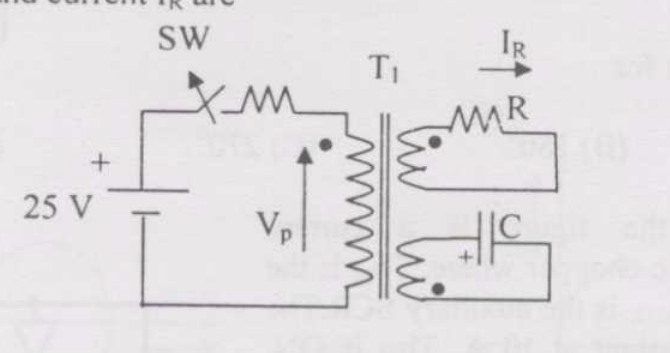
\includegraphics[scale=0.5]{figs/fig 6.png}
	\label{Fig-6}
\end{figure}
\begin{enumerate}
\item $-25 V, 0.0 A$
\item very large voltage, very large current
\item $5.0 V, 0.5 A$
\item $-5.0 V, -5.0 A$
\end{enumerate}

\item IC $555$ in the adjacent figure is configured as an astable
multivibrator. it is enabled to oscillate at $t=0$ by applying a high input to pin 4. The pin description is: 1 and 8-supply; 2-trigger; 4-reset; 6-threshold; 7-discharge. The waveform appearing across the capacitor starting from $t=0$, as observed on a storage CRO is:
\begin{figure}[h]
	\centering
	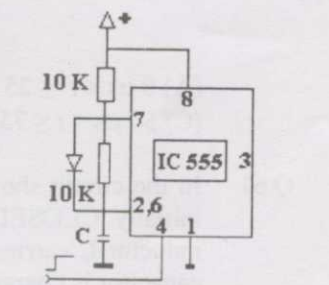
\includegraphics[scale=0.5]{figs/fig 7.png}
	\label{Fig-7}
\end{figure}
\begin{enumerate}
\item 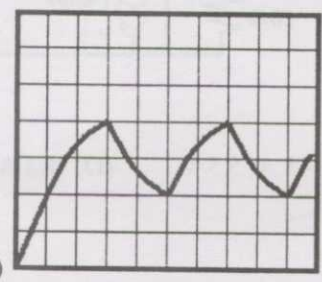
\includegraphics[width=5cm]{figs/fig 7.1.png}
\item 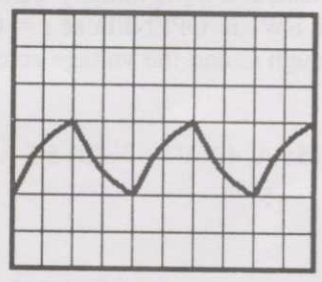
\includegraphics[width=5cm]{figs/fig 7.2.png}
\item 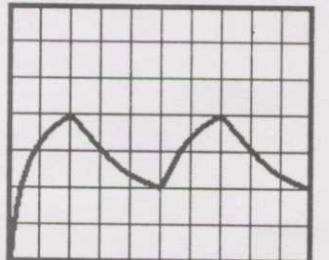
\includegraphics[width=5cm]{figs/fig 7.3.png}
\item 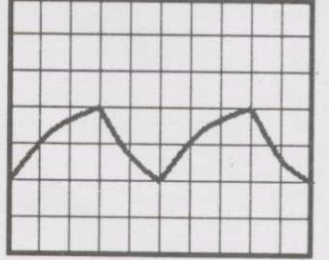
\includegraphics[width=5cm]{figs/fig 7.4.png}
\end{enumerate}
\item In the circuit figure the diode connects the ac source to a pure inductance L. The diode conducts for
\begin{figure}[h]
	\centering
	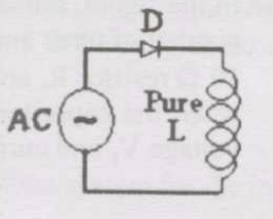
\includegraphics[scale=0.5]{figs/fig 8.png}
	\label{Fig-7}
\end{figure}
\begin{enumerate}
\item $90 \degree$
\item $180 \degree$
\item $270 \degree$
\item $360 \degree$
\end{enumerate}

\item The circuit in the figure is a current commutated dc-dc chopper where, $Th_M$ is the main SCR and $Th_{AUX}$ is the auxiliary SCR. The load current is constant at $10$ A. $Th_M$ is turned OFF between
\begin{figure}[h]
	\centering
	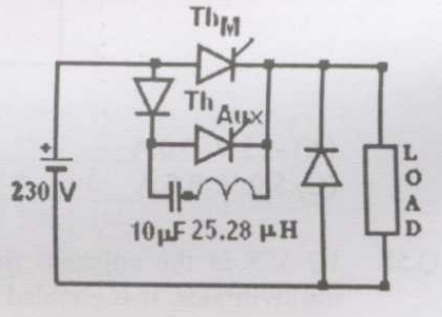
\includegraphics[scale=0.5]{figs/fig 9.png}
	\label{Fig-7}
\end{figure}
\begin{enumerate}
\item $0 \mu s<t\leq 25 \mu s$
\item $25 \mu s<t\leq 50 \mu s$
\item $50 \mu s<t\leq 75 \mu s$
\item $75 \mu s<t\leq100\mu s$
\end{enumerate}
\item In the circuit shown in figure switch $SW_1$ is initially CLOSED and $SW_2$ is OPEN. The inductor L carries a current of 10 A and the capacitor is charged to 10 V with polarities as indicated. $SW_2$ is initially CLOSED at $t=0-$ and $SW_1$ is OPENED at $t=0$. The current through C and the voltage across L at $t=0+$ is
\begin{figure}[h]
	\centering
	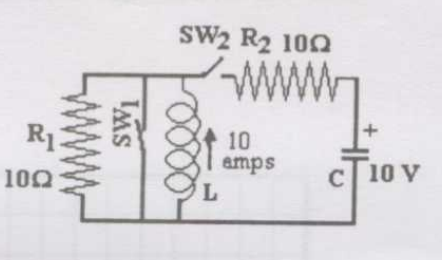
\includegraphics[scale=0.5]{figs/fig 10.png}
	\label{Fig-7}
\end{figure}
\begin{enumerate}
\item $55 A, 4.5 V$
\item $5.5 A, 45 V$
\item $45 A, 5.5 V$
\item $4.5 A, 55V$
\end{enumerate}
\item The R-L-C series circuit shown is supplied from a variable frequency voltage source. The admittance-locus of the R-L-C network at terminals AB for increasing frequency $w$ is
\begin{figure}[h]
	\centering
	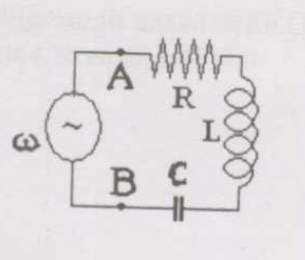
\includegraphics[scale=0.5]{figs/fig 11.png}
	\label{Fig-7}
\end{figure}
\begin{enumerate}
\item 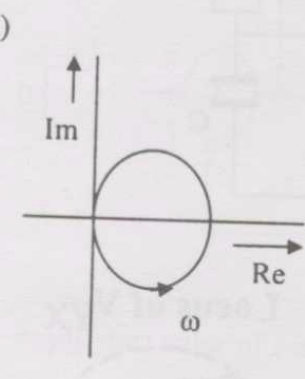
\includegraphics[width=5cm]{figs/fig 11.1.png}
\item 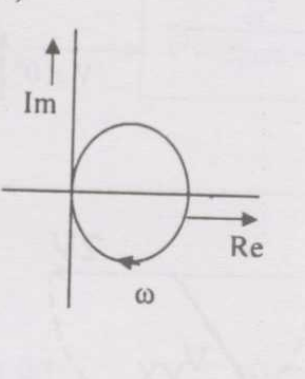
\includegraphics[width=5cm]{figs/fig 11.2.png}
\item 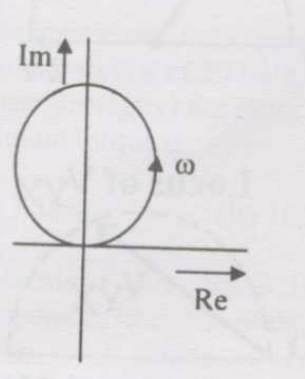
\includegraphics[width=5cm]{figs/fig 11.3.png}
\item 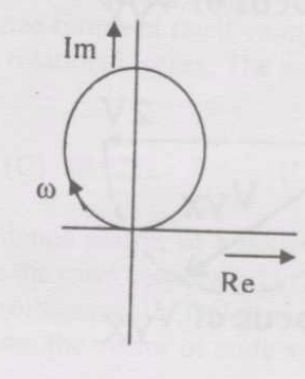
\includegraphics[width=5cm]{figs/fig 11.4.png}
\end{enumerate}

\item In the figure given below all phasors are with reference to the potential at point "O". The locus of voltage phasor $\mathbf{V_{YX}}$ as R is varied from zero to infinity is shown by
\begin{figure}[h]
	\centering
	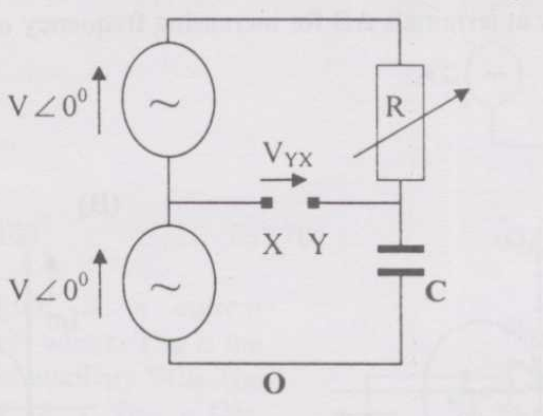
\includegraphics[scale=0.5]{figs/fig 12.png}
	\label{Fig-7}
\end{figure}
\begin{enumerate}
\item 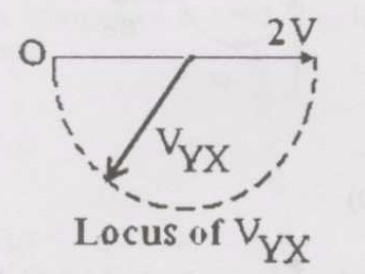
\includegraphics[width=5cm]{figs/fig 12.1.png}
\item 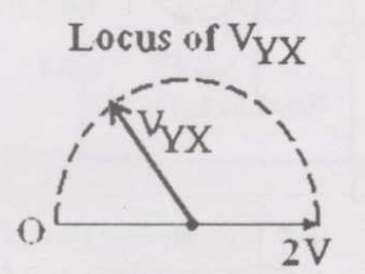
\includegraphics[width=5cm]{figs/fig 12.2.png}
\item 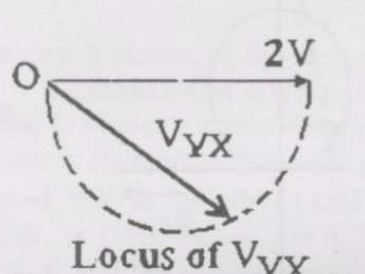
\includegraphics[width=5cm]{figs/fig 12.3.png}
\item 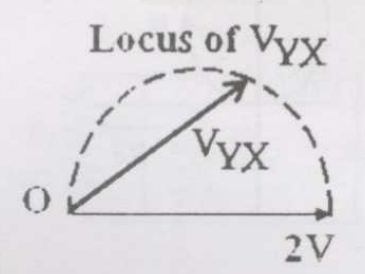
\includegraphics[width=5cm]{figs/fig 12.4.png}
\end{enumerate}

\item A 3 V dc supply with an internal resistance of $2 \ohm$ supplies a passive non-linear resistance characterized by the relation $V_{NL}=I_{NL}^2$. The power dissipated in the non-linear resistance is
\begin{enumerate}
\item $1.0 W$
\item $1.5 W$
\item $2.5 W$
\item $3.0 W$
\end{enumerate}

\item Consider the feedback control system shown below which is subjected to a unit step input. The system is stable and has the following parameters $k_P = 4, K_1 = 10, w=500 $ and $\epsilon = 0.7$. The steady state value of $z$ is.
\begin{figure}[h]
	\centering
	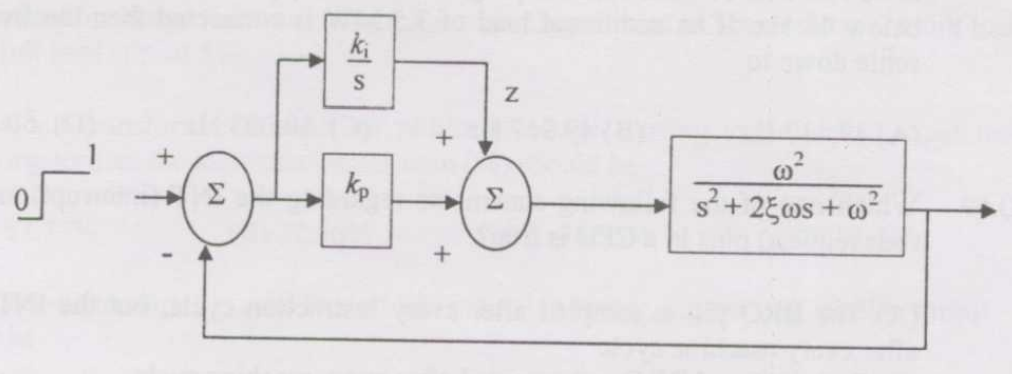
\includegraphics[scale=0.5]{figs/fig 14.png}
	\label{Fig-7}
\end{figure}
\begin{enumerate}
\item $1$
\item $0.25$
\item $0.1$
\item $0$
\end{enumerate}

\item A three-phase squirrel cage induction motor has a starting torque of 
$150\%$ and a maximum torque of $300\%$ with respect to rated torque at rated voltage and rated frequency. Neglect the stator resistance and rotational losses. The value of slip for maximum torque is   

\begin{enumerate}
\item $13.48\%$
\item $16.24\%$
\item $18.92\%$
\item $26.79\%$
\end{enumerate}

\item The matrix A given below is the node incidence matrix of a network. The columns correspond to branches of the network while the rows correspond to nodes. Let $V=[\begin{matrix}v_{1}&v_{2}&...v_{6}\end{matrix}]^{T}$ denote the vector of branch voltages while $I=[i_{1}i_{2}...i_{6}]^{T}$ that of branch currents. The vector $E=[\begin{matrix}e_{1}&e_{2}&e_{3}&e_{4}\end{matrix}]^{T}$ denotes the vector of node voltages relative to a common ground.   

\[
A = \begin{bmatrix}
1 & 1 & 1 & 0 & 0 & 0 \\
0 & -1 & 0 & -1 & 1 & 0 \\
-1 & 0 & 0 & 0 & -1 & -1 \\
0 & 0 & -1 & 1 & 0 & 1
\end{bmatrix}
\]

Which of the following statements is true?

\begin{enumerate}
\item The equations $v_{1}-v_{2}+v_{3}=0$ , $v_{3}+v_{4}-v_{5}=0$ are KVL equations for the network for some loops
\item The equations $v_{1}-v_{3}-v_{6}=0] [v_{4}+v_{5}-v_{6}=0$ are KVL equations for the network for some loops
\item $E=AV$
\item $AV=0$ are KVL equations for the network
\end{enumerate}

\item An isolated $50$ Hz synchronous generator is rated at $15 MW$, which is also the maximum continuous power limit of its prime mover. It is equipped with a speed governor with $5\%$ droop. Initially, the generator is feeding three loads of $4 MW$ each at $50$ Hz. One of these loads is programmed to trip permanently if the frequency falls below $48 Hz$. If an additional load of $3.5 MW$ is connected, then the frequency will settle down to   
\begin{enumerate}
\item $49.417 Hz$
\item $49.917 Hz$
\item $50.083 Hz$
\item $50.583 Hz$
\end{enumerate}
\end{enumerate} 
\end{document}

